\begin{savequote}[75mm]
The artist works with forms. Forms are  present everywhere: in space, on the earth, in fauna, in society. They're close to musical form, so we have to be able to `read' them, to understand them — only thus can we work conciously  and create something really new. For that we have to know not only the forms of the present but also those that existed in the past.
\qauthor{Iannis Xenakis\footnote{\citet[126]{xenakis-interviews}}}
\end{savequote}

\chapter{\textit{Akasha} (2015) by Trevor Bača}
\label{Chapter2}
% \lettrine[lines=2,slope=-2pt,nindent=2pt]{\textcolor{SchoolColor}{I}}{ first met}

\lettrine[lines=3]{\setmainfont{GoudyInitialen}[Path=./fonts/, Extension = .ttf]\color{printGreen}I}{ first met} Trevor Ba\v{c}a (b.1975) around 2015 when a small organization for the performance of new music in Cincinnati, Ohio, where I had been studying Violoncello Performance and Music Composition at the University of Cincinnati, contacted me in order to give the United States premiere of Bača's 2013 cello work \textit{Traiettorie inargentate}. We corresponded over the course of a few weeks, exchanging emails of rehearsal recordings and performance notes, and eventually I gave the concert. Afterwards, I received an email containing the score of the then newly composed \textit{Akasha} for string quartet. I have taken a great interest in Bača's work ever since, and these two pieces in particular hold a very special place because of their dramatic contrast, beautiful colors, formal articulation, and inventive structuring.

\textit{Akasha} features a formal approach similar to that of Guerrero. Several musical materials are introduced in sequence and developed independently of one another. These different materials are identifiable by characteristic behaviors and a tight coupling between rhythmic, harmonic, and timbral elements of sound. In order to study the large-scale formal characteristics of this work, it is required to have an ability to distinguish these multi-parametric materials.

\section{Materials}

The sketches for \textit{Akasha} begin with the definition of distinct material-types which drive the development of the work.

\begin{table}[H]
    \myfloatalign
    \begin{tabularx}{\textwidth}{lllll} \toprule
        \tableheadline{Type A} & \tableheadline{Type B} & \tableheadline{Type C} & \tableheadline{Type D} & \tableheadline{Type E} \\
        \midrule
        legg. staccati &  polyphony & trills & sustained & on bridge \\
        minor 2\textsuperscript{nds} & quarter tones & whole tone & A partials & tone-less \\
        \midrule
        ascent & ritardando & fragment $\rightarrow$ cluster & static $\rightarrow$ activated & static/noise $\rightarrow$\\
        & & & & active/pitched\\
        \bottomrule
    \end{tabularx}
    \caption[Summary of materials in \textit{Akasha}]{Summary of materials in \textit{Akasha}}
    \label{tab:akasha-material-table}
\end{table}

These five materials are very well-defined; the following descriptions come from sketch materials which are reproduced in Appendix \vref{AppendixC}. While the sketches list material manifestations in an order of often accumulating transformation, they are not necessarily deployed linearly within the final composition.

\subsection{Material A}

The most recognizeable form of material \boxed{\text{A}} are the leggierissimo off-sting staccati found at the beginning of the piece. By observing the outline for the available manifestations of this material we can already see an example of a material which is developed non-linearly in the score. In his outline of material manifestations, Bača describes material \boxed{\text{A}} as beginning as isolated notes with scratch tone; increasing to non-scratch gettati; increasing in density; then disintegrating into gettato bursts surrounded by silence. This material also gradually ascends in register through a looping transposition of a basic pitch sequence. The sketches describe a primarily \lilyDynamics{pp} dynamic, but dynamics vary in the final piece.

\subsection{Material B}

The sketches label material \boxed{\text{B}} as a ``microtonal field.'' This material opens with solo melodic gestures, gradually increasing from two-voice to four-voice polyphony. Material manifestations four through seven (as numbered in the sketches) alternate between two static chords, one with semitone intonation and the other with quartertone intonation, with different bow speeds ranging from \ac{SB}, essentially producing a scratch tone, to \ac{XFB}, which produces an animated flautando-like timbre. The final manifestations of material \boxed{\text{B}} take the form of rallantandi on the semitone chord played \ac{SB}, which each diminuendo.

\subsection{Material C}

Sketches outlining material \boxed{\text{C}} takes a slightly different form in the finished composition when compared with the sketch outlining the materials. The sketches describe material \boxed{\text{C}} as ``massed trills'' developing from isolated trills; to grouped trill figures; to longer phrases with intermittent pauses; to a cycle of ``3-note tenuti, trill loops without breaks, and fluid/mechanical block dynamics''; concluding as a fixed trill field on a four-note chord. These gestures operate as an irregular trill with increasing and decreasing speed.

\subsection{Material D}

The sketches label material \boxed{\text{D}} as a ``spectral field,'' emphasizing a static voicing of natural harmonics across the ensemble. The chord is constructed from harmonics of the A strings of the instruments; string IV on both the viola and the violoncello is retuned from the original C down to A, thus increasing the number of natural harmonics of that shared fundamental. The violoncello is assigned the 9\textsuperscript{th} harmonic; the viola is assigned the 7\textsuperscript{th}; violin 2 the 6\textsuperscript{th}; and violin 1 the 5\textsuperscript{th}. In the finished score, this appears to have been changed to 11\textdegree-7\textdegree-5\textdegree-9\textdegree, with the first and second violins swapping occasionally. This results in a final notated chord of approximately D\mynatural5-G\myquarterflat5-C\mysharp7-B\mynatural7. These pitches are naturally tuned, thus standing apart from the equal-tempered sounds of the other materials. The available manifestations of this material are described as d1: a detuned octave between the viola and violoncello; d2: tutti detuned octaves; d3: viola and violoncello with harmonics 7 and 9; d4: tutti arco 9\textdegree-7\textdegree-6\textdegree-5\textdegree; d5: tutti 9\textdegree-7\textdegree-6\textdegree-5\textdegree with trills; d6: tutti 9\textdegree-7\textdegree-6\textdegree-5\textdegree trills with envelopes of tasto to ponticello motion; and d7: \ac{XSP} swipes against spectral chord. The trajectory of this material is a gradual enlivening of color while preserving a static harmonic field; however, not every one of these manifestations of the material appears in the final work.

\subsection{Material E}

Material \boxed{\text{E}} comprises white noise sounds produced by bowing directly on the bridge, or by gradually drifting off and on the bridge. The scale of bridge positions is \ac{XSP}, $\frac{1}{4}$ \ac{OB}, $\frac{1}{2}$ \ac{OB}, $\frac{3}{4}$ \ac{OB}, and completely \ac{OB}. The seven available manifestations of this material show a gradual change from static bowing on the bridge, to which rhythmic activity is added; to increased variability of the bridge position; to the addition of glissando figures when the bow is in the \ac{XSP} position. Once ordered in the piece, the narrative arc of this material is a gradual emergence of clarity and activity out of static noise.

\section{Formal Permutations}

\textit{Akasha's} form concatenates four main sequences derived from a basic progression of eleven moments. A moment is defined by the composing-out of one or more materials, as specified by the formal diagram described below. The main line of material in figure \ref{tab:moments-1} is in the center. The top and bottom lines show companion material; there is no hierarchy between them. There appears to be no combinatorial system or set of permutations from which this progression was produced; however, the materials are introduced in alphabetical order. This series of eleven moments is partitioned into sections:

\begin{table}[H]
    % \centering
\resizebox{!}{40pt}{
\begin{tabular}{ c | c c c c c | c c | c c c c}
sections & [02] &  &  &  &  & [03] &  & [04] &  &  &  \\  
  moments & \textcolor{red}{2} & \textcolor{red}{3} & \textcolor{red}{4} & \textcolor{red}{5} & \textcolor{red}{6} & \textcolor{red}{7} & \textcolor{red}{8} & \textcolor{red}{9} & \textcolor{red}{10} & \textcolor{red}{11} & \textcolor{red}{12} \\
  measures & 4-8 & 9-13 & 14-19 & 20-21 & 21-23 & 24-32 & 33-34 & 35-42 & 43-49 & 50 & 51-58  \\  
  \midrule
 materials & &  &  &  &  & A &  &  & A &  &  \\  
 & A & B & B & C & A & B & C & D & D & A & E \\ 
 & B &  & C &  & C & C & D &  & E & E &  \\  
\end{tabular}
}
\caption{\textit{Akasha} moments, part 1}
    \label{tab:moments-1}
\end{table}

Transpositions are applied to the sequence of materials such that \boxed{\text{A}} becomes \boxed{\text{C}}, \boxed{\text{B}} becomes \boxed{\text{D}}, etc.:

\begin{figure}[H]
    \centering
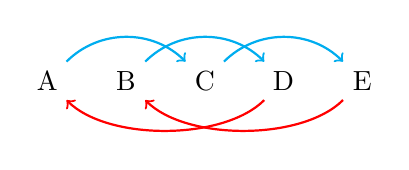
\begin{tikzpicture}
    \node(1) {A};
    \node[right of=1] (2) {B};
    \node[right of=2] (3) {C};
    \node[right of=3] (4) {D};
    \node[right of=4] (5) {E};
    \draw[->, thick]
    (1) edge[cyan, out=45, in=135, looseness=1,] (3)
    (2) edge[cyan, out=45, in=135, looseness=1,] (4)
    (3) edge[cyan, out=45, in=135, looseness=1,] (5)
    (4) edge[red, out=-135, in=-45, looseness=0.75,] (1)
    (5) edge[red, out=-135, in=-45, looseness=0.75,] (2)
;

\end{tikzpicture}
    \caption{Material transpositions}
    \label{fig:akasha-material-transposition-1}
\end{figure}

This operation is equivalent to +2 from the basic form with a modulus of five, such that materials transposed higher than the available 5 wrap back around to the beginning of the material set. The moments are repartitioned into new sections of different sizes:

\begin{table}[H]
    % \centering
    \resizebox{!}{40pt}{
\begin{tabular}{ c | c | c c c c c | c c | c c c}
 sections & ([04]) & [05] &  &  &  &  & [06] &  & [07] &  &  \\  
 moments & \textcolor{red}{13} & \textcolor{red}{14} & \textcolor{red}{15} & \textcolor{red}{16} & \textcolor{red}{17} & \textcolor{red}{18} & \textcolor{red}{19} & \textcolor{red}{20} & \textcolor{red}{21} & \textcolor{red}{22} & \textcolor{red}{23} \\
 measures & 59-61 & 62-70 & 71-93 & 94-98 & 99-103 & 104-112 & 113-151 &  & 152-161 & 162-173  &  174-186 \\  
 \midrule
materials &  &  &  &  &  & C &  &  & C &  &  \\  
 & C & D & D & E & C & D & E & A & A & C & B \\ 
 & D &  & E &  & E & E & A &  & B & B &  \\  
\end{tabular}
}
\caption{\textit{Akasha} moments, part 2}
    \label{tab:moments-2}
\end{table}

Transpositions are applied once more. Materials in blue represent materials which Bača replaces in a later step:

\begin{table}[H]
    % \centering
    \resizebox{!}{27.2pt}{
\begin{tabular}{ c | c c | c c c | c | c c c c | c}
 sections & ([07]) &  & [08] &  &  & [09] & [10] &  &  &  & [12] \\
 \midrule
 materials & &  &  &  &  & \textcolor{printBlue}{E} &  &  & \textcolor{printBlue}{E} &  &  \\  
&  E & A & A & B & E & \textcolor{printBlue}{A} & \textcolor{printBlue}{B} & \textcolor{printBlue}{C} & \textcolor{printBlue}{C} & \textcolor{printBlue}{E} & \textcolor{printBlue}{D} \\ 
&  A &  & B &  & B & \textcolor{printBlue}{B} & \textcolor{printBlue}{C} &  & \textcolor{printBlue}{D} & \textcolor{printBlue}{D} &  \\  
\end{tabular}
}
 \caption{\textit{Akasha} moments, part 3 (original)}
    \label{tab:moments-3-a}
\end{table}

The transpositions are applied once again and the moments are repartitioned:

\begin{table}[H]
    % \centering
    \resizebox{!}{40pt}{
\begin{tabular}{ c | c c c c | c c | c c | c c c}
sections & ([12]) &  &  &  & [13] &  & [14] &  & [15] &  &  \\  
moments &  \textcolor{red}{35} & \textcolor{red}{36} & \textcolor{red}{37} & \textcolor{red}{38} & \textcolor{red}{39} & \textcolor{red}{40} & \textcolor{red}{41} & \textcolor{red}{42} & \textcolor{red}{43} & \textcolor{red}{44} & \textcolor{red}{45} \\
measures & (265-333) &  &  &  & 334-339 &  & 340-368 &  & 369-393 &  &  \\
\midrule
materials &  &  &  &  &  & \colorbox{yellow}{B} &  &  & \colorbox{yellow}{B} &  &  \\  
& B & C & C & D & B & \colorbox{yellow}{C} & \colorbox{yellow}{D} & \colorbox{yellow}{E} & \colorbox{yellow}{E} & \colorbox{yellow}{B} & \colorbox{yellow}{A} \\ 
& C &  & D &  & D & \colorbox{yellow}{D} & \colorbox{yellow}{E} &  & \colorbox{yellow}{A} & \colorbox{yellow}{A} &  \\  
\end{tabular}
}
 \caption{\textit{Akasha} moments, part 4}
    \label{tab:moments-4}
\end{table}

Finally, the materials in sections 9-12 are replaced by their transpositional equivalents derived in figure \ref{tab:moments-4}, indicated in yellow:

\begin{table}[H]
    % \centering
    \resizebox{!}{40pt}{
\begin{tabular}{ c | c c | c c c | c | c c c c | c}
 sections & ([07]) &  & [08] &  &  & [09] & [10] &  &  &  & [12] \\  
 moments & \textcolor{red}{24} & \textcolor{red}{25} & \textcolor{red}{26} & \textcolor{red}{27} & \textcolor{red}{28} & \textcolor{red}{29} & \textcolor{red}{30} & \textcolor{red}{31} & \textcolor{red}{32} & \textcolor{red}{33} & \textcolor{red}{35} \\
 measures & 187-195 & 196-199 & 200-203 & 204-213 & 214-216 & 117-223 & 224-239 & 240-243 & 244-253 & 254-260 & 265-333 \\
 \midrule
 materials & &  &  &  &  & \colorbox{yellow}{B} &  &  & \colorbox{yellow}{B} &  &  \\  
&  E & A & A & B & E & \colorbox{yellow}{C} & \colorbox{yellow}{D} & \colorbox{yellow}{E} & \colorbox{yellow}{E} & \colorbox{yellow}{B} & \colorbox{yellow}{A} \\ 
&  A &  & B &  & B & \colorbox{yellow}{D} & \colorbox{yellow}{E} &  & \colorbox{yellow}{A} & \colorbox{yellow}{A} &  \\  
\end{tabular}
}
 \caption{\textit{Akasha} moments, part 3 (with substitution)}
    \label{tab:moments-3-b}
\end{table}

The sections represent distinct passages of compositional effort, ultimately forming the basis of \textit{Akasha}'s 15 sections. After the completion of the moment diagram (as attested by the version history of the section files found on GitHub\footnote{\url{https://github.com/}}), Bača added the opening gesture of material \boxed{\text{E}} to this structure, perhaps to soften the opening. Bača also inserted a section before what would originally have been called section eleven,\footnote{The inserted section eleven comprises moment 34 from measures 261-264 on material \boxed{\text{A}}, recollecting, as previously stated, the start of section six.} with an exact quotation of material found in section six. After designing this ordering of the materials, Bača then wrote an outline of the work, featuring written descriptions of each musical gesture. This storyboard describes the sequence of every event in the piece.

\section{Time Signature Series}

Time signature analysis reveals a pattern of alternation between two different types of time signature in the piece. The generative process for each series is defined; then, each series is rotated for every section of the piece at regular intervals of rotation. As described in Appendix \vref{helianthus}, Bača rotates the outer and inner layers as in \autoref{lst:sigs}, with reversed rotations of -1 and 1. Because helianthation produces a nested list of sublists, the section-specific time signature rotation refers to the sublist on which the time signatures begin. The other feature of the time signature series, common to Bača's other works, is monotonic increase of integers in each sublist.

\begin{lstlisting}[language=Python,frame=tb,caption={Definition of time signatures in \textit{Akasha}},label=lst:sigs]
def _time_signature_series():
    time_signature_series = dict()
    numerators = [[3, 3, 4, 5], [4, 6, 6]]
    groups = baca.sequence.helianthate(numerators, -1, 1)
    assert len(groups) == 24
    lengths = [len(_) for _ in groups]
    numerators = abjad.sequence.flatten(groups, depth=-1)
    _time_signatures = [abjad.TimeSignature((_, 4)) for _ in numerators]
    groups = abjad.sequence.partition_by_counts(_time_signatures, lengths)
    time_signature_series["A"] = groups
    numerators = [[3, 6, 7, 7], [4, 8, 9, 9], [3, 4]]
    groups = baca.sequence.helianthate(numerators, -1, 1)
    assert len(groups) == 36
    lengths = [len(_) for _ in groups]
    numerators = abjad.sequence.flatten(groups, depth=-1)
    _time_signatures = [abjad.TimeSignature((_, 8)) for _ in numerators]
    groups = abjad.sequence.partition_by_counts(_time_signatures, lengths)
    time_signature_series["B"] = groups
    return time_signature_series
\end{lstlisting}

\subsection{Time Signature Series A}

Time signature series A is defined as the sequence $[[3, 3, 4, 5], [4, 6, 6]]$ and its collection of helianthations, accumulated to identity. This series is used in sections 2, 4, 6, 7, 9, 10, 11, 13, and 14 of the piece. For each section, the series is rotated by 0, 3, 6, 9, 12, 15, 6, 18, and 21, representing a continuous rotation by three. Section eleven features a different rotation because this section flashes back to section six as an exact recurrence. The numbers produced by this series are treated as numerators of time signatures over denominators of \lilyText{4}.

\begin{lstlisting}[language=Python,frame=tb,caption={Enumeration of helianthated rotations of time signature series A},label=lst:sigs-a]
>>> numerators = [[3, 3, 4, 5], [4, 6, 6]]
>>> groups = baca.sequence.helianthate(numerators, -1, 1)
>>> partitions = abjad.sequence.partition_by_counts(groups, [2], cyclic=True)
>>> for partition in partitions:
...     print(partition)
...
[[3, 3, 4, 5], [4, 6, 6]]
[[6, 4, 6], [5, 3, 3, 4]]
[[4, 5, 3, 3], [6, 6, 4]]
[[4, 6, 6], [3, 4, 5, 3]]
[[3, 3, 4, 5], [6, 4, 6]]
[[6, 6, 4], [5, 3, 3, 4]]
[[4, 5, 3, 3], [4, 6, 6]]
[[6, 4, 6], [3, 4, 5, 3]]
[[3, 3, 4, 5], [6, 6, 4]]
[[4, 6, 6], [5, 3, 3, 4]]
[[4, 5, 3, 3], [6, 4, 6]]
[[6, 6, 4], [3, 4, 5, 3]]
\end{lstlisting}

\begin{table}[H]
    \centering
    \resizebox{\columnwidth}{!}{
    \begin{tabular}{ c c l }
 Section & Index of rotation & Time signatures \\ 
 \toprule
 2 & 0 & \lilyTimeSignature{3}{4}, \lilyTimeSignature{3}{4}, \lilyTimeSignature{4}{4}, \lilyTimeSignature{5}{4}, \lilyTimeSignature{4}{4}, \lilyTimeSignature{6}{4}, \lilyTimeSignature{6}{4}, \lilyTimeSignature{6}{4}, \lilyTimeSignature{4}{4}, \lilyTimeSignature{6}{4}, \lilyTimeSignature{5}{4}, \lilyTimeSignature{3}{4} \\  
 % \midrule
 \vspace{0.25mm} \\
 4 & 3 & \lilyTimeSignature{6}{4}, \lilyTimeSignature{4}{4}, \lilyTimeSignature{6}{4}, \lilyTimeSignature{6}{4}, \lilyTimeSignature{6}{4}, \lilyTimeSignature{4}{4}, \lilyTimeSignature{3}{4}, \lilyTimeSignature{4}{4}, \lilyTimeSignature{5}{4}, \lilyTimeSignature{3}{4}, \lilyTimeSignature{3}{4}, \lilyTimeSignature{3}{4}, \lilyTimeSignature{4}{4}, \lilyTimeSignature{5}{4}, \lilyTimeSignature{4}{4}, \lilyTimeSignature{6}{4}, \lilyTimeSignature{6}{4} \\ 
 % \midrule
 \vspace{0.25mm} \\
 6 & 6 & \lilyTimeSignature{4}{4}, \lilyTimeSignature{6}{4}, \lilyTimeSignature{6}{4}, \lilyTimeSignature{5}{4}, \lilyTimeSignature{3}{4}, \lilyTimeSignature{3}{4}, \lilyTimeSignature{4}{4}, \lilyTimeSignature{4}{4}, \lilyTimeSignature{5}{4}, \lilyTimeSignature{3}{4}, \lilyTimeSignature{3}{4}, \lilyTimeSignature{6}{4}, \lilyTimeSignature{4}{4}, \lilyTimeSignature{6}{4}, \lilyTimeSignature{6}{4}, \lilyTimeSignature{6}{4}, \lilyTimeSignature{4}{4}, \lilyTimeSignature{3}{4}, \lilyTimeSignature{4}{4}, \lilyTimeSignature{5}{4}, \lilyTimeSignature{3}{4}, \lilyTimeSignature{3}{4}, \lilyTimeSignature{3}{4}, \lilyTimeSignature{4}{4}, \lilyTimeSignature{5}{4}, \lilyTimeSignature{4}{4}, \lilyTimeSignature{6}{4}, \lilyTimeSignature{6}{4}, \lilyTimeSignature{6}{4}, \lilyTimeSignature{4}{4}, \lilyTimeSignature{6}{4}, \lilyTimeSignature{5}{4}, \lilyTimeSignature{3}{4}, \lilyTimeSignature{3}{4} \\ 
  % \midrule
  \vspace{0.25mm} \\
 7 & 9 & \lilyTimeSignature{3}{4}, \lilyTimeSignature{4}{4}, \lilyTimeSignature{5}{4}, \lilyTimeSignature{3}{4}, \lilyTimeSignature{3}{4}, \lilyTimeSignature{3}{4}, \lilyTimeSignature{4}{4}, \lilyTimeSignature{5}{4}, \lilyTimeSignature{6}{4}, \lilyTimeSignature{6}{4}, \lilyTimeSignature{4}{4}, \lilyTimeSignature{4}{4}, \lilyTimeSignature{6}{4}, \lilyTimeSignature{6}{4}, \lilyTimeSignature{5}{4}, \lilyTimeSignature{3}{4}, \lilyTimeSignature{3}{4}, \lilyTimeSignature{4}{4}, \lilyTimeSignature{4}{4}, \lilyTimeSignature{5}{4}, \lilyTimeSignature{3}{4}, \lilyTimeSignature{3}{4}, \lilyTimeSignature{6}{4}, \lilyTimeSignature{4}{4}, \lilyTimeSignature{6}{4}, \lilyTimeSignature{6}{4}, \lilyTimeSignature{6}{4}, \lilyTimeSignature{4}{4}, \lilyTimeSignature{3}{4}, \lilyTimeSignature{4}{4}, \lilyTimeSignature{5}{4}, \lilyTimeSignature{3}{4}, \lilyTimeSignature{3}{4}, \lilyTimeSignature{3}{4}, \lilyTimeSignature{4}{4}, \lilyTimeSignature{5}{4}, \lilyTimeSignature{4}{4}, \lilyTimeSignature{6}{4}, \lilyTimeSignature{6}{4}, \lilyTimeSignature{6}{4} \\ 
  % \midrule
  \vspace{0.25mm} \\
 9 & 12 & \lilyTimeSignature{4}{4}, \lilyTimeSignature{5}{4}, \lilyTimeSignature{3}{4}, \lilyTimeSignature{3}{4}, \lilyTimeSignature{4}{4} \\ 
  % \midrule
  \vspace{0.25mm} \\
 10 & 15 & \lilyTimeSignature{6}{4}, \lilyTimeSignature{4}{4}, \lilyTimeSignature{6}{4}, \lilyTimeSignature{6}{4}, \lilyTimeSignature{6}{4}, \lilyTimeSignature{4}{4}, \lilyTimeSignature{5}{4}, \lilyTimeSignature{3}{4}, \lilyTimeSignature{3}{4}, \lilyTimeSignature{4}{4}, \lilyTimeSignature{4}{4}, \lilyTimeSignature{5}{4}, \lilyTimeSignature{3}{4}, \lilyTimeSignature{3}{4}, \lilyTimeSignature{4}{4}, \lilyTimeSignature{6}{4}, \lilyTimeSignature{6}{4}, \lilyTimeSignature{6}{4}, \lilyTimeSignature{4}{4}, \lilyTimeSignature{6}{4}, \lilyTimeSignature{3}{4}, \lilyTimeSignature{4}{4}, \lilyTimeSignature{5}{4}, \lilyTimeSignature{3}{4}, \lilyTimeSignature{3}{4}, \lilyTimeSignature{3}{4}, \lilyTimeSignature{4}{4}, \lilyTimeSignature{5}{4}, \lilyTimeSignature{6}{4}, \lilyTimeSignature{6}{4}, \lilyTimeSignature{4}{4}, \lilyTimeSignature{4}{4}, \lilyTimeSignature{6}{4} \\ 
  % \midrule
  \vspace{0.25mm} \\
 11 & 6 & \lilyTimeSignature{4}{4}, \lilyTimeSignature{6}{4}, \lilyTimeSignature{6}{4} \\ 
  % \midrule
  \vspace{0.25mm} \\
 13 & 18 & \lilyTimeSignature{4}{4}, \lilyTimeSignature{6}{4}, \lilyTimeSignature{6}{4}, \lilyTimeSignature{3}{4} \\ 
  % \midrule
  \vspace{0.25mm} \\
 14 & 21 & \lilyTimeSignature{5}{4}, \lilyTimeSignature{3}{4}, \lilyTimeSignature{3}{4}, \lilyTimeSignature{4}{4}, \lilyTimeSignature{4}{4}, \lilyTimeSignature{5}{4}, \lilyTimeSignature{3}{4}, \lilyTimeSignature{3}{4}, \lilyTimeSignature{6}{4}, \lilyTimeSignature{6}{4}, \lilyTimeSignature{4}{4}, \lilyTimeSignature{4}{4}, \lilyTimeSignature{6}{4}, \lilyTimeSignature{6}{4}, \lilyTimeSignature{3}{4}, \lilyTimeSignature{4}{4}, \lilyTimeSignature{5}{4}, \lilyTimeSignature{3}{4}, \lilyTimeSignature{3}{4}, \lilyTimeSignature{3}{4}, \lilyTimeSignature{4}{4}, \lilyTimeSignature{5}{4}, \lilyTimeSignature{6}{4}, \lilyTimeSignature{4}{4}, \lilyTimeSignature{6}{4}, \lilyTimeSignature{6}{4}, \lilyTimeSignature{6}{4}, \lilyTimeSignature{4}{4} \\ 
 \bottomrule
\end{tabular}
}
    \caption{Time signature series A}
    \label{fig:series-a-table}
\end{table}

\subsection{Time Signature Series B}

Time signature series B is defined as the sequence $[[3, 6, 7, 7], [4, 8, 9, 9], [3, 4]]$ and its sequence of helianthations, accumulated to identity with denominators of \lilyText{8}. This time signature series is used in sections 1, 3, 5, 8, 12, 15 with rotations of 0, 6, 12, 18, 24, 30, respectively.

\begin{lstlisting}[language=Python,frame=tb,caption={Enumeration of helianthated rotations of time signature series B},label=lst:sigs-b]
>>> numerators = [[3, 6, 7, 7], [4, 8, 9, 9], [3, 4]]
>>> groups = baca.sequence.helianthate(numerators, -1, 1)
>>> partitions = abjad.sequence.partition_by_counts(groups, [3], cyclic=True)
>>> for partition in partitions:
...     print(partition)
...
[[3, 6, 7, 7], [4, 8, 9, 9], [3, 4]]
[[9, 4, 8, 9], [4, 3], [7, 3, 6, 7]]
[[3, 4], [7, 7, 3, 6], [9, 9, 4, 8]]
[[6, 7, 7, 3], [8, 9, 9, 4], [4, 3]]
[[4, 8, 9, 9], [3, 4], [3, 6, 7, 7]]
[[4, 3], [7, 3, 6, 7], [9, 4, 8, 9]]
[[7, 7, 3, 6], [9, 9, 4, 8], [3, 4]]
[[8, 9, 9, 4], [4, 3], [6, 7, 7, 3]]
[[3, 4], [3, 6, 7, 7], [4, 8, 9, 9]]
[[7, 3, 6, 7], [9, 4, 8, 9], [4, 3]]
[[9, 9, 4, 8], [3, 4], [7, 7, 3, 6]]
[[4, 3], [6, 7, 7, 3], [8, 9, 9, 4]]
\end{lstlisting}

\begin{table}[H]
    \centering
    \resizebox{\columnwidth}{!}{
    \begin{tabular}{ c c l }
 Section & Index of rotation & Time signatures \\ 
 \toprule
 1 & 0 & \lilyTimeSignature{3}{8}, \lilyTimeSignature{6}{8} \\  
 % \midrule
 \vspace{0.25mm} \\
 3 & 6 & \lilyTimeSignature{9}{8}, \lilyTimeSignature{9}{8}, \lilyTimeSignature{4}{8}, \lilyTimeSignature{8}{8}, \lilyTimeSignature{3}{8}, \lilyTimeSignature{4}{8}, \lilyTimeSignature{7}{8}, \lilyTimeSignature{7}{8} \\
 % \midrule
 \vspace{0.25mm} \\
 5 & 12 & \lilyTimeSignature{3}{8}, \lilyTimeSignature{4}{8}, \lilyTimeSignature{3}{8}, \lilyTimeSignature{6}{8}, \lilyTimeSignature{7}{8}, \lilyTimeSignature{7}{8}, \lilyTimeSignature{4}{8}, \lilyTimeSignature{8}{8}, \lilyTimeSignature{9}{8}, \lilyTimeSignature{9}{8}, \lilyTimeSignature{7}{8}, \lilyTimeSignature{3}{8}, \lilyTimeSignature{6}{8}, \lilyTimeSignature{7}{8}, \lilyTimeSignature{9}{8}, \lilyTimeSignature{4}{8}, \lilyTimeSignature{8}{8}, \lilyTimeSignature{9}{8}, \lilyTimeSignature{4}{8}, \lilyTimeSignature{3}{8}, \lilyTimeSignature{9}{8}, \lilyTimeSignature{9}{8}, \lilyTimeSignature{4}{8}, \lilyTimeSignature{8}{8}, \lilyTimeSignature{3}{8}, \lilyTimeSignature{4}{8}, \lilyTimeSignature{7}{8}, \lilyTimeSignature{7}{8}, \lilyTimeSignature{3}{8}, \lilyTimeSignature{6}{8}, \lilyTimeSignature{4}{8}, \lilyTimeSignature{3}{8}, \lilyTimeSignature{6}{8}, \lilyTimeSignature{7}{8}, \lilyTimeSignature{7}{8}, \lilyTimeSignature{3}{8}, \lilyTimeSignature{8}{8}, \lilyTimeSignature{9}{8}, \lilyTimeSignature{9}{8}, \lilyTimeSignature{4}{8}, \\
 & & \lilyTimeSignature{3}{8}, \lilyTimeSignature{6}{8}, \lilyTimeSignature{7}{8}, \lilyTimeSignature{7}{8} \\
 % \midrule
 \vspace{0.25mm} \\
 8 & 18 & \lilyTimeSignature{7}{8}, \lilyTimeSignature{7}{8}, \lilyTimeSignature{3}{8}, \lilyTimeSignature{6}{8}, \lilyTimeSignature{9}{8}, \lilyTimeSignature{9}{8}, \lilyTimeSignature{4}{8}, \lilyTimeSignature{8}{8}, \lilyTimeSignature{3}{8}, \lilyTimeSignature{4}{8}, \lilyTimeSignature{8}{8}, \lilyTimeSignature{9}{8}, \lilyTimeSignature{9}{8}, \lilyTimeSignature{4}{8}, \lilyTimeSignature{4}{8}, \lilyTimeSignature{3}{8} \\
 % \midrule
 \vspace{0.25mm} \\
 12 & 24 & \lilyTimeSignature{4}{8}, \lilyTimeSignature{8}{8}, \lilyTimeSignature{9}{8}, \lilyTimeSignature{9}{8}, \lilyTimeSignature{3}{8}, \lilyTimeSignature{4}{8}, \lilyTimeSignature{3}{8}, \lilyTimeSignature{6}{8}, \lilyTimeSignature{7}{8}, \lilyTimeSignature{7}{8}, \lilyTimeSignature{4}{8}, \lilyTimeSignature{3}{8}, \lilyTimeSignature{7}{8}, \lilyTimeSignature{3}{8}, \lilyTimeSignature{6}{8}, \lilyTimeSignature{7}{8}, \lilyTimeSignature{9}{8}, \lilyTimeSignature{4}{8}, \lilyTimeSignature{8}{8}, \lilyTimeSignature{9}{8}, \lilyTimeSignature{7}{8}, \lilyTimeSignature{7}{8}, \lilyTimeSignature{3}{8}, \lilyTimeSignature{6}{8}, \lilyTimeSignature{9}{8}, \lilyTimeSignature{9}{8}, \lilyTimeSignature{4}{8}, \lilyTimeSignature{8}{8}, \lilyTimeSignature{3}{8}, \lilyTimeSignature{4}{8}, \lilyTimeSignature{8}{8}, \lilyTimeSignature{9}{8}, \lilyTimeSignature{9}{8}, \lilyTimeSignature{4}{8}, \lilyTimeSignature{4}{8}, \lilyTimeSignature{3}{8}, \lilyTimeSignature{6}{8}, \lilyTimeSignature{7}{8}, \lilyTimeSignature{7}{8}, \lilyTimeSignature{3}{8}, \\
 & & \lilyTimeSignature{3}{8}, \lilyTimeSignature{4}{8}, \lilyTimeSignature{3}{8}, \lilyTimeSignature{6}{8}, \lilyTimeSignature{7}{8}, \lilyTimeSignature{7}{8}, \lilyTimeSignature{4}{8}, \lilyTimeSignature{8}{8}, \lilyTimeSignature{9}{8}, \lilyTimeSignature{9}{8}, \lilyTimeSignature{7}{8}, \lilyTimeSignature{3}{8}, \lilyTimeSignature{6}{8}, \lilyTimeSignature{7}{8}, \lilyTimeSignature{9}{8}, \lilyTimeSignature{4}{8}, \lilyTimeSignature{8}{8}, \lilyTimeSignature{9}{8}, \lilyTimeSignature{4}{8}, \lilyTimeSignature{3}{8}, \lilyTimeSignature{9}{8}, \lilyTimeSignature{9}{8}, \lilyTimeSignature{4}{8}, \lilyTimeSignature{8}{8} \\
 % \midrule
 \vspace{0.25mm} \\
 15 & 30 & \lilyTimeSignature{3}{8}, \lilyTimeSignature{4}{8}, \lilyTimeSignature{7}{8}, \lilyTimeSignature{7}{8}, \lilyTimeSignature{3}{8}, \lilyTimeSignature{6}{8}, \lilyTimeSignature{9}{8}, \lilyTimeSignature{9}{8}, \lilyTimeSignature{4}{8}, \lilyTimeSignature{8}{8}, \lilyTimeSignature{6}{8}, \lilyTimeSignature{7}{8}, \lilyTimeSignature{7}{8}, \lilyTimeSignature{3}{8}, \lilyTimeSignature{8}{8}, \lilyTimeSignature{9}{8}, \lilyTimeSignature{9}{8}, \lilyTimeSignature{4}{8}, \lilyTimeSignature{4}{8}, \lilyTimeSignature{3}{8}, \lilyTimeSignature{4}{8}, \lilyTimeSignature{8}{8}, \lilyTimeSignature{9}{8}, \lilyTimeSignature{9}{8} \\
 \bottomrule
\end{tabular}
}
    \caption{Time signature series B}
    \label{fig:series-b-table}
\end{table}

After defining the process by which time signatures are arranged in each section, Bača chooses the number of measures for each section. Some measures are selected to be a silent grand pause; these are inserted between time signatures, visually compressed, and given a fermata.

\section{Sections 1-6}

Here I describe the opening 6 sections of \textit{Akasha}.

\begin{table}[H]
    % \centering
    \begin{tabular}{c|l}
        Section & Measures \\
        \toprule
        1 & 1-3 \\
        2 & 4-23 \\ 
        3 & 24-34 \\ 
        4 & 35-61 \\ 
        5 & 62-112 \\ 
        6 & 113-151 \\ 
    \end{tabular}
    \caption{Sections 1-6 in \textit{Akasha}}
    \label{tab:akasha-1-6-measures}
\end{table}

\subsection{Section 1}

The work begins with a sputtering, interruptive exposition where the different materials are fairly easy to distinguish from one another. Section 1 consists of a single note of the viola bowing on the bridge at \lilyDynamics{mf}, followed by a very long fermata. %This insertion causes the work to begin with material \boxed{\text{E}} instead of the originally planned \boxed{\text{A}}.

% \begin{figure}[H]
%     \includegraphics[scale=0.75]{lilypond/akasha_01.pdf}
%     \caption{Section 1 of \textit{Akasha} Annotated}
%     \label{fig:akasha-1}
% \end{figure}

\subsection{Section 2}

The \textbf{2\textsuperscript{nd}} moment, in measures 4-8, corresponds to materials \boxed{\text{AB}} interpreted as a sequential statement. The cello, playing \boxed{\text{B}}, has rhythms derived from a talea of durations $\frac{7}{16}$, $\frac{1}{16}$, $\frac{10}{16}$, and $\frac{2}{16}$:

\begin{figure}[H]
    \includegraphics{lilypond/section_2/akasha_cello_1.pdf}
    \caption{Cello; measures 4-5; score}
    \label{fig:cello-talea}
\end{figure}

The rhythms of the second violin and viola, playing \boxed{\text{A}}, are also derived from a talea of 32\textsuperscript{nd} notes:

\setcounter{figure}{7}
\setcounter{subFigure}{1}
\renewcommand{\thefigure}{\thechapter.\arabic{figure}.\alph{subFigure}}
\begin{figure}[H]
    \includegraphics{lilypond/section_2/akasha_violin_viola_step_1.pdf}
    \caption{Violin 2 and viola; measure 7; stage 1}
    \label{fig:violin-viola-talea-1}
\end{figure}

One extra count is included in each quarter note subdivision:

% \setcounter{figure}{7}
% \setcounter{subFigure}{2}
% \begin{figure}[H]
%     \includegraphics{lilypond/section_2/akasha_violin_viola_step_2.pdf}
%     \caption{Violin 2 and viola; measure 7; stage 2}
%     \label{fig:violin-viola-talea-2}
% \end{figure}

% The measure is subdivided into quarter note durations:

\setcounter{figure}{7}
\setcounter{subFigure}{2}
\begin{figure}[H]
    \includegraphics{lilypond/section_2/akasha_violin_viola_step_3.pdf}
    \caption{Violin 2 and viola; measure 7; stage 2}
    \label{fig:violin-viola-talea-3}
\end{figure}

Over a period of 36 notes, only attacks 0, 1, 2, 12, 13, 21, 31, 32, and 33 are heard:

\setcounter{figure}{7}
\setcounter{subFigure}{3}
\begin{figure}[H]
    \includegraphics{lilypond/section_2/akasha_violin_viola_step_4.pdf}
    \caption{Violin 2 and viola; measure 7; stage 3}
    \label{fig:violin-viola-talea-4}
\end{figure}

In the case of the second violin, all tuplets except for the first two are silenced, while the viola silences all but the last:

\setcounter{figure}{7}
\setcounter{subFigure}{4}
\begin{figure}[H]
    \includegraphics{lilypond/section_2/akasha_violin_viola_step_5.pdf}
    \caption{Violin 2 and viola; measure 7; stage 4}
    \label{fig:violin-viola-talea-5}
\end{figure}

Empty tuplets are respelled as rests:

\setcounter{figure}{7}
\setcounter{subFigure}{5}
\begin{figure}[H]
    \includegraphics{lilypond/section_2/akasha_violin_viola_step_5_score.pdf}
    \caption{Violin 2 and viola; measure 7; score}
    \label{fig:violin-viola-talea-5-score}
\end{figure}

The \textbf{3\textsuperscript{rd}} moment, in measures 9-13, corresponds to the materials \boxed{\text{B(A)}} interpreted as a sequential statement, with an overlap. Here material \boxed{\text{A}} has been reintroduced despite the original map containing only \boxed{\text{B}}. The \boxed{\text{B}} rhythms in both violins and the viola are produced with the same methodology as the cello (figure \ref{fig:cello-talea}), only with substituted duration numerators and occasional rotation. The talea consists of durations $\frac{4}{16}$, $\frac{14}{16}$, $\frac{4}{16}$, $\frac{6}{16}$, $\frac{18}{16}$:

\setcounter{figure}{8}
\setcounter{subFigure}{1}
% \renewcommand{\thefigure}{\thechapter.\arabic{figure}}
\begin{figure}[H]
% \resizebox{\columnwidth}{!}{
    \includegraphics{lilypond/section_2/polyphony_1.pdf}
    % }
    \caption{Violins and viola; measures 9-10; stage 1}
    \label{fig:polyphony-talea-1}
\end{figure}

Violin 1 silences all notes except those at index 0, 1, 2. Violin 2 silences all notes except those at index 2, 3, 4. The viola silences all notes except those at index 1, 2, 3. This produces a slightly staggered entrance and exit of each voice, but preserves rhythmic unison:

\setcounter{figure}{8}
\setcounter{subFigure}{2}
\begin{figure}[H]
% \resizebox{\columnwidth}{!}{
    \includegraphics{lilypond/section_2/polyphony_2.pdf}
    % }
    \caption{Violins and viola; measures 9-10; score}
    \label{fig:polyphony-talea-2}
\end{figure}

After the fermata (m. 11), \boxed{\text{B}} is moved to the lower trio of violin 2, viola, and cello, with a rotation of -2, producing $\frac{4}{16}$, $\frac{6}{16}$, $\frac{18}{16}$, $\frac{4}{16}$, $\frac{14}{16}$:

\setcounter{figure}{9}
\setcounter{subFigure}{1}
\begin{figure}[H]
% \resizebox{\columnwidth}{!}{
    \includegraphics{lilypond/section_2/polyphony_3.pdf}
    % }
    \caption{Violin 2, viola, and cello; measure 12; stage 1}
    \label{fig:polyphony-talea-3}
\end{figure}

Violin 2 silences all but indices 1, 2, and 3. The viola, also with a rotation of -2, silences all but indices 2, 3, and 4. The cello, with a rotation of -2, silences all but indices 0, 1, and 2. This produces the same effect of staggered entrances and exits with coincident attacks:

\setcounter{figure}{9}
\setcounter{subFigure}{2}
\begin{figure}[H]
% \resizebox{\columnwidth}{!}{
    \includegraphics{lilypond/section_2/polyphony_4.pdf}
    % }
    \caption{Violin 2, viola, and cello; measure 12; score}
    \label{fig:polyphony-talea-4}
\end{figure}

The first violin, now playing material \boxed{\text{A}}, produces the same rhythms as the first appearance of \boxed{\text{A}} in the second violin and viola:

\setcounter{figure}{10}
\setcounter{subFigure}{1}
\begin{figure}[H]
% \resizebox{\columnwidth}{!}{
    \includegraphics{lilypond/section_2/gettato_3.pdf}
    % }
    \caption{Violin 1; measure 12; stage 1}
    \label{fig:gettato-v1-1}
\end{figure}

All but the last two tuplets are silenced:

\setcounter{figure}{10}
\setcounter{subFigure}{2}
\begin{figure}[H]
% \resizebox{\columnwidth}{!}{
    \includegraphics{lilypond/section_2/gettato_4.pdf}
    % }
    \caption{Violin 1; measure 12; stage 2}
    \label{fig:gettato-v1-4}
\end{figure}

Empty tuplets are respelled as rests:

\setcounter{figure}{10}
\setcounter{subFigure}{3}
\begin{figure}[H]
% \resizebox{\columnwidth}{!}{
    \includegraphics{lilypond/section_2/gettato_4_score.pdf}
    % }
    \caption{Violin 1; measure 12; score}
    \label{fig:gettato-v1-4-score}
\end{figure}

The \textbf{4\textsuperscript{th}} moment, in measures 14-19, corresponds to the materials \boxed{\text{BC}} interpreted as an overlapping statement. Material \boxed{\text{B}} in the viola, with a rotation of -4 is accompanied by the cello, with a rotation of -6. This produces a duet with individual taleas of ($\frac{18}{16}$, $\frac{4}{16}$, $\frac{14}{16}$, $\frac{4}{16}$, $\frac{6}{16}$) and ($\frac{14}{16}$, $\frac{4}{16}$, $\frac{6}{16}$, $\frac{18}{16}$, $\frac{4}{16}$):

\setcounter{figure}{11}
\setcounter{subFigure}{1}
\renewcommand{\thefigure}{\thechapter.\arabic{figure}}
\begin{figure}[H]
% \resizebox{\columnwidth}{!}{
    \includegraphics{lilypond/section_2/duet_1.pdf}
    % }
    \caption{Viola and cello; measures 14-16; score}
    \label{fig:duet-1}
\end{figure}

This begins the development of a continuous rotation pattern, where each appearance of material \boxed{\text{B}} in the viola is rotated two positions to the left, and the cello is rotated four positions to the left. After the fermata, the viola and cello rhythms are rotated to their final position of -8 and -10 respectively. This produces a duet with individual taleas of ($\frac{6}{16}$, $\frac{18}{16}$, $\frac{4}{16}$, $\frac{14}{16}$, $\frac{4}{16}$) and ($\frac{4}{16}$, $\frac{14}{16}$, $\frac{4}{16}$, $\frac{6}{16}$, $\frac{18}{16}$):

\setcounter{figure}{12}
\begin{figure}[H]
% \resizebox{\columnwidth}{!}{
    \includegraphics{lilypond/section_2/duet_2.pdf}
    % }
    \caption{Viola and cello; measure 18; score}
    \label{fig:duet-2}
\end{figure}

As for the violins' \boxed{\text{C}} material, the accelerandi\footnote{For a description of the accelerando interpolation process, see \vref{rmakers}.} alternates between interpolations from $\frac{1}{2}$ to $\frac{1}{8}$ and $\frac{1}{8}$ to $\frac{1}{2}$. The total duration of the musical event is factored into the interpolation equation and the resulting accelerandi alternate between one measure and two measures in duration. Interpolations from short durations to longer durations are front-loaded to produce more attacks in a rallantando than an accelerando:

\setcounter{figure}{13}
\setcounter{subFigure}{1}
\renewcommand{\thefigure}{\thechapter.\arabic{figure}.\alph{subFigure}}
\begin{figure}[H]
% \resizebox{\columnwidth}{!}{
    \includegraphics{lilypond/section_2/acc_1.pdf}
    % }
    \caption{Violins; measures 14-16; stage 1}
    \label{fig:accelerando-1}
\end{figure}

The first violin silences all attacks except for -11, -10, -8, -6, -4, -2, and -1. The second violin's rhythm reverses the ordering of the accelerando/rallantando gestures and silences all but attacks -10, -8, -7, -5, -3, -2, and -1:

\setcounter{figure}{13}
\setcounter{subFigure}{2}
\begin{figure}[H]
% \resizebox{\columnwidth}{!}{
    \includegraphics{lilypond/section_2/acc_2.pdf}
    % }
    \caption{Violins; measures 14-16; stage 2}
    \label{fig:accelerando-2}
\end{figure}

Empty tuplets are respelled as rests:

\setcounter{figure}{13}
\setcounter{subFigure}{3}
\begin{figure}[H]
% \resizebox{\columnwidth}{!}{
    \includegraphics{lilypond/section_2/acc_2_score.pdf}
    % }
    \caption{Violins; measures 14-16; score}
    \label{fig:accelerando-2-score}
\end{figure}

Despite sharing nearly identical rest-forcing patterns, the opposing accelerando directions result in a lack of coincident attacks. In measure 18,\footnote{Fermatas are numbered as measures in the score.} the violins produce accelerandi identical to the previous measures, but revealing previously silenced opening gestures:

\setcounter{figure}{14}
\setcounter{subFigure}{1}
\begin{figure}[H]
% \resizebox{\columnwidth}{!}{
    \includegraphics{lilypond/section_2/acc_3.pdf}
    % }
    \caption{Violins; measure 18; stage 1}
    \label{fig:accelerando-3}
\end{figure}

Violin 1 silences all but 0, 2, 3, and -1, while violin 2 silences all but 0, 1, 4, and -1:

\setcounter{figure}{14}
\setcounter{subFigure}{2}
\renewcommand{\thefigure}{\thechapter.\arabic{figure}.\alph{subFigure}}
\begin{figure}[H]
% \resizebox{\columnwidth}{!}{
    \includegraphics{lilypond/section_2/acc_4.pdf}
    % }
    \caption{Violins; measure 18; score}
    \label{fig:accelerando-4}
\end{figure}

The \textbf{5\textsuperscript{th}} moment, in measures 20-21, develops material \boxed{\text{C}}. The violins play alone, with identical rhythms, but with a reversal of roles. Both violins silence all notes except those at indices 0, 2, and -1:

% \begin{figure}[H]
% % \resizebox{\columnwidth}{!}{
%     \includegraphics{lilypond/section_2/acc_5.pdf}
%     % }
%     \caption{Accelerando 5}
%     \label{fig:accelerando-5}
% \end{figure}

\setcounter{figure}{15}
\setcounter{subFigure}{0}
\renewcommand{\thefigure}{\thechapter.\arabic{figure}}
\begin{figure}[H]
% \resizebox{\columnwidth}{!}{
    \includegraphics{lilypond/section_2/acc_6.pdf}
    % }
    \caption{Violins; measure 20; score}
    \label{fig:accelerando-6}
\end{figure}

The \textbf{6\textsuperscript{th}} moment, in measures 22-23, interprets materials \boxed{\text{AC}} as a concurrent statement. Violin 2 uses the ritardando pattern with silences applied to all but 0, 1, -1:

\setcounter{figure}{16}
\begin{figure}[H]
% \resizebox{\columnwidth}{!}{
    \includegraphics{lilypond/section_2/acc_8.pdf}
    % }
    \caption{Violin 2; measure 22; score}
    \label{fig:accelerando-8}
\end{figure}

The cello takes up the 32\textsuperscript{nd}-note rhythms described above:

\setcounter{figure}{17}
\setcounter{subFigure}{1}
\renewcommand{\thefigure}{\thechapter.\arabic{figure}.\alph{subFigure}}
\begin{figure}[H]
% \resizebox{\columnwidth}{!}{
    \includegraphics{lilypond/section_2/gett_1.pdf}
    % }
    \caption{Cello; measure 22; stage 1}
    \label{fig:final-gett-1}
\end{figure}

The first and last tuplets are silenced:

\setcounter{figure}{17}
\setcounter{subFigure}{2}
\begin{figure}[H]
% \resizebox{\columnwidth}{!}{
    \includegraphics{lilypond/section_2/gett_2.pdf}
    % }
    \caption{Cello; measure 22; stage 2}
    \label{fig:final-gett-2}
\end{figure}

Empty tuplets are respelled as rests:

\setcounter{figure}{17}
\setcounter{subFigure}{3}
\begin{figure}[H]
% \resizebox{\columnwidth}{!}{
    \includegraphics{lilypond/section_2/gett_2_score.pdf}
    % }
    \caption{Cello; measure 22; score}
    \label{fig:final-gett-2-score}
\end{figure}

An examination of the pitch content of this section of the score reveals characteristic harmonic traits associated with each material. \boxed{\text{A}} uses semitones with a tendency toward neighbor-note motion. \boxed{\text{B}} makes use of quarter tones and mostly stepwise motion with contrary voice-leading. \boxed{\text{C}} takes the form of a highly slowed-down trill, so each voice only oscillates between two pitches. This version of the pitch material of \boxed{\text{C}} produces a whole-tone effect.

% \begin{figure}[H]
% \resizebox{\columnwidth}{!}{
%     \includegraphics{lilypond/akasha_02.pdf}
%     }
%     \caption{Section 2 of \textit{Akasha} Annotated}
%     \label{fig:akasha-2}
% \end{figure}

\subsection{Section 3}

The \textbf{7\textsuperscript{th}} moment, in measures 24-32, deploys the compound material \boxed{\text{ABC}}. Violin 1 performs an accelerando from material \boxed{\text{C}} on single measures. All notes are silenced except 0, 2, and 3:

\setcounter{figure}{18}
\setcounter{subFigure}{0}
\renewcommand{\thefigure}{\thechapter.\arabic{figure}}
\begin{figure}[H]
% \resizebox{\columnwidth}{!}{
    \includegraphics{lilypond/section_3/accel_1.pdf}
    % }
    \caption{Violin 1; measure 24; score}
    \label{fig:section-3-accel}
\end{figure}

The rhythm of \boxed{\text{B}} material is derived from the previous rhythms in violin 2 and in the viola with a rotation of -2 and silences for the first two note durations. This produces a duet of individual taleas of ($\frac{4}{16}$, $\frac{14}{16}$, $\frac{4}{16}$, $\frac{6}{16}$, $\frac{18}{16}$) and ($\frac{4}{16}$, $\frac{6}{16}$, $\frac{18}{16}$, $\frac{4}{16}$, $\frac{14}{16}$):

\setcounter{figure}{19}
\begin{figure}[H]
% \resizebox{\columnwidth}{!}{
    \includegraphics{lilypond/section_3/section_3_polyphony_1.pdf}
    % }
    \caption{Violin 2 and viola; measures 24-26; score}
    \label{fig:section-3-accel-2}
\end{figure}

The cello's first, four-measure statement of \boxed{\text{A}} deploys a variation on the 32\textsuperscript{nd}-note rhythms developed in section two. These rhythms are made through the creation of two patterns: one with indices 0, 1, 2, 3 with a period of 12 and another with the same indices with a period of 20:

\setcounter{figure}{20}
\setcounter{subFigure}{1}
\renewcommand{\thefigure}{\thechapter.\arabic{figure}.\alph{subFigure}}
\begin{figure}[H]
% \resizebox{\columnwidth}{!}{
    \includegraphics{lilypond/section_3/section_3_pattern_1.pdf}
    % }
    \caption{Cello; measures 24-27; stage 1; pattern 1}
    \label{fig:section-3-pattern-1}
\end{figure}

\setcounter{figure}{20}
\setcounter{subFigure}{2}
\begin{figure}[H]
% \resizebox{\columnwidth}{!}{
    \includegraphics{lilypond/section_3/section_3_pattern_2.pdf}
    % }
    \caption{Cello; measures 24-27; stage 1; pattern 2}
    \label{fig:section-3-pattern-2}
\end{figure}

The union of these patterns is taken:

\setcounter{figure}{20}
\setcounter{subFigure}{3}
\begin{figure}[H]
% \resizebox{\columnwidth}{!}{
    \includegraphics{lilypond/section_3/section_3_pattern_intersection.pdf}
    % }
    \caption{Cello; measures 24-27; stage 2}
    \label{fig:section-3-pattern-intersection}
\end{figure}

The union is inverted, such that notes become rests and rests become notes:

\setcounter{figure}{20}
\setcounter{subFigure}{4}
\begin{figure}[H]
% \resizebox{\columnwidth}{!}{
    \includegraphics{lilypond/section_3/section_3_inverted_intersection.pdf}
    % }
    \caption{Cello; measures 24-27; stage 3}
    \label{fig:section-3-inverted-intersection}
\end{figure}

Extra counts are cyclically applied to each quarter note subdivision with a pattern of $[1, 1, 0, 2]$:

% \begin{figure}[H]
% % \resizebox{\columnwidth}{!}{
%     \includegraphics{lilypond/section_3/section_3_extra_counts_pattern.pdf}
%     % }
%     \caption{Cello; measures 24-27; stage 4}
%     \label{fig:section-3-pattern-extra-counts}
% \end{figure}

% The measures are subdivided into quarter notes:

\setcounter{figure}{20}
\setcounter{subFigure}{5}
\begin{figure}[H]
% \resizebox{\columnwidth}{!}{
    \includegraphics{lilypond/section_3/section_3_preprocessed.pdf}
    % }
    \caption{Cello; measures 24-27; stage 4}
    \label{fig:section-3-pattern-partitioned}
\end{figure}

All tuplets are silenced except 5, -6, -5, -4, -3, -2, and -1:

\setcounter{figure}{20}
\setcounter{subFigure}{6}
\begin{figure}[H]
% \resizebox{\columnwidth}{!}{
    \includegraphics{lilypond/section_3/section_3_silenced_tuplets.pdf}
    % }
    \caption{Cello; measures 24-27; stage 5}
    \label{fig:section-3-pattern-silences}
\end{figure}

Empty tuplets are respelled as rests:

\setcounter{figure}{20}
\setcounter{subFigure}{7}
\begin{figure}[H]
% \resizebox{\columnwidth}{!}{
    \includegraphics{lilypond/section_3/section_3_silenced_tuplets_score.pdf}
    % }
    \caption{Cello; measures 24-27; score}
    \label{fig:section-3-pattern-silences-score}
\end{figure}

These pattern-handling processes are illustrated in listing \ref{lst:gettato-pattern}.

\begin{lstlisting}[frame=tb,caption={Gettato attack patterns, measures 24-27},label=lst:gettato-pattern]
>>> import abjad
>>> pattern_1 = abjad.index([0, 1, 2, 3], 12)
>>> pattern_2 = abjad.index([0, 1, 2, 3], 20)
>>> pattern_3 = pattern_1 | pattern_2
>>> pattern_4 = ~pattern_3
>>> print(pattern_1.get_boolean_vector())
[1, 1, 1, 1, 0, 0, 0, 0, 0, 0, 0, 0]
>>> print(pattern_2.get_boolean_vector())
[1, 1, 1, 1, 0, 0, 0, 0, 0, 0, 0, 0, 0, 0, 0, 0, 0, 0, 0, 0]
>>> print(pattern_3.get_boolean_vector())
[1, 1, 1, 1, 0, 0, 0, 0, 0, 0, 0, 0, 1, 1, 1, 1, 0, 0, 0, 0, 1, 1, 1, 1, 1, 1, 1, 1, 0, 0, 0, 0, 0, 0, 0, 0, 1, 1, 1, 1, 1, 1, 1, 1, 0, 0, 0, 0, 1, 1, 1, 1, 0, 0, 0, 0, 0, 0, 0, 0]
>>> print(pattern_4.get_boolean_vector())
[0, 0, 0, 0, 1, 1, 1, 1, 1, 1, 1, 1, 0, 0, 0, 0, 1, 1, 1, 1, 0, 0, 0, 0, 0, 0, 0, 0, 1, 1, 1, 1, 1, 1, 1, 1, 0, 0, 0, 0, 0, 0, 0, 0, 1, 1, 1, 1, 0, 0, 0, 0, 1, 1, 1, 1, 1, 1, 1, 1]
\end{lstlisting}

This boolean vector of the intersected patterns is taken as a stream of 32\textsuperscript{nd} notes where the 0 values represent rests and the 1 values represent sounding attacks. The next statement has a rotation of -4 and extra counts of $[1, 1, 0, 2]$:

% \setcounter{figure}{21}
% \setcounter{subFigure}{1}
% \begin{figure}[H]
% % \resizebox{\columnwidth}{!}{
%     \includegraphics{lilypond/section_3/pattern_fragment_no_rotation.pdf}
%     % }
%     \caption{Cello; measure 29; stage 1}
%     \label{fig:section-3-pattern-1-no-rotation}
% \end{figure}

\setcounter{figure}{21}
\setcounter{subFigure}{0}
\renewcommand{\thefigure}{\thechapter.\arabic{figure}}
\begin{figure}[H]
% \resizebox{\columnwidth}{!}{
    \includegraphics{lilypond/section_3/pattern_fragment_rotation_minus_4.pdf}
    % }
    \caption{Cello; measure 29; score}
    \label{fig:section-3-pattern-minus-4}
\end{figure}

The final statement of this moment rotates -4 once more, resulting in -8, and keeps the same extra count sequence. No tuplets are silenced in these two brief gestures:

% \setcounter{figure}{22}
% \setcounter{subFigure}{1}
% \begin{figure}[H]
% % \resizebox{\columnwidth}{!}{
%     \includegraphics{lilypond/section_3/pattern_fragment_2_no_rotation.pdf}
%     % }
%     \caption{Cello; measure 31; stage 1}
%     \label{fig:section-3-pattern-2-no-rotation}
% \end{figure}

\setcounter{figure}{22}
\setcounter{subFigure}{0}
\renewcommand{\thefigure}{\thechapter.\arabic{figure}}
\begin{figure}[H]
% \resizebox{\columnwidth}{!}{
    \includegraphics{lilypond/section_3/pattern_fragment_2_rotation_minus_8.pdf}
    % }
    \caption{Cello; measure 31; score}
    \label{fig:section-3-pattern-minus-8}
\end{figure}

The \textbf{8\textsuperscript{th}} moment, in measures 33-34, develops \boxed{\text{CD}}. Violin 2 uses the \boxed{\text{C}} accelerando with the note at index 3 forced to a rest. The viola and cello begin their duet of \boxed{\text{D}}, which will be developed in the next section. This material begins simply by filling the final measure of section 3 with one note equal to the total duration of the measure.

Material \boxed{\text{C}} continues the whole-tone trills and \boxed{\text{B}} has quarter tone voice-leading. \boxed{\text{D}} develops as a glissando drifting downward toward the octave, and it can be seen that this section begins the process in the next section without the downward motion. \boxed{\text{B}}, on the other hand, articulates pitches which follow a strict pattern. First, an integer sequence is given as [0, 1, 0, -1, -2, 0, -1, 0, 1, 3, 2, 1, 0, 2, 3, 4, 3, 5, 6, 4, 5], constituting the basic intervalic contour:

\setcounter{figure}{23}
\setcounter{subFigure}{0}
\renewcommand{\thefigure}{\thechapter.\arabic{figure}}
\begin{figure}[H]
% \resizebox{\columnwidth}{!}{
    \includegraphics{lilypond/gett_intervals_1.pdf}
    % }
    \caption{Ascending interval pattern used in material \boxed{\text{A}}}
    \label{fig:gett-intervals-1}
\end{figure}

Bača uses both the original form and an inverted form of the sequence to produce ascending or descending pitches. Bača also transposes the sequence by a starting pitch. A list of pitch integers is constructed by adding the starting pitch number to every number of the interval series. To invert the sequence for a downward gesture, Bača adds a negative version of each the interval value to the starting pitch, resulting in an inverted pitch fragment. After deriving these basic pitches for material \boxed{\text{A}}, they are applied to every note; when the sequence is consumed, the sequence is transposed and continues. In this moment, Bača uses the inverted form of the interval series; the interval of transposition used is -3, or down three semitones, and a starting pitch of -2 is given, or B\myflat3. So, the inverted interval series is [0, -1, 0, 1, 2, 0, 1, 0, -1, -3, -2, -1, 0, -2, -3, -4, -3, -5, -6, -4, -5], when transposed by the starting pitch become [-2, -3, -2, -1, 0, -2, -1, -2, -3, -5, -4, -3, -2, -4, -5, -6, -5, -7, -8, -6, -7], and resulting in the first transposition being [-5, -6, -5, -4, -3, -5, -4, -5, -6, -8, -7, -6, -5, -7, -8, -9, -8, -10, -11, -9, -10]:

\setcounter{figure}{24}
\begin{figure}[H]
% \resizebox{\columnwidth}{!}{
    \includegraphics{lilypond/gett_intervals_2.pdf}
    % }
    \caption{Descending interval pattern with transposition of -3 used in material \boxed{\text{A}} in measures 25-31}
    \label{fig:gett-intervals-2}
\end{figure}

% \begin{figure}[H]
% \resizebox{\columnwidth}{!}{
%     \includegraphics{lilypond/akasha_03.pdf}
%     }
%     \caption{Section 3 of \textit{Akasha} Annotated}
%     \label{fig:akasha-3}
% \end{figure}

\subsection{Section 4}

The \textbf{9\textsuperscript{th}} moment, the continuation of \boxed{\text{D}}, appears in measures 35-42. For each non-fermata measure, the cello produces a duration of the length of the measure, and the viola uses a partitioning process in which each measure is given two notes with a proportional relationship of \( 8\hspace{-1mm}:\hspace{-1mm}1 \):\footnote{For more information on this partitioning process, see \vref{rmakers}.}

\setcounter{figure}{25}
\begin{figure}[H]
% \resizebox{\columnwidth}{!}{
    \includegraphics{lilypond/section_4/section_4_tuplets_1.pdf}
    % }
    \caption{Viola and cello; measures 35-41; score}
    \label{fig:section-4-partitioning}
\end{figure}

The viola and cello elide their statement of \boxed{\text{D}} into the next moment (mm. 43-49). This \textbf{10\textsuperscript{th}} moment develops \boxed{\text{ADE}}. The viola fills the first four measures with individual notes, and the cello fills the same with a tied note of the total duration of these measures:

\setcounter{figure}{26}
\begin{figure}[H]
% \resizebox{\columnwidth}{!}{
    \includegraphics{lilypond/section_4/section_4_duet_2.pdf}
    % }
    \caption{Viola and cello; measures 43-46; score}
    \label{fig:section-4-notes-v-tie}
\end{figure}

As counterpoint to this, the violins fill the first five measures of this moment with a long, tied note representing \boxed{\text{E}}. The moment ends with a single-measure burst of \boxed{\text{A}} in the cello. The cello's rhythms are constructed with the same logic as the previous section, with an extra count series of 1, 1, 0, and 2, and a rotation of -12:

\setcounter{figure}{27}
\begin{figure}[H]
% \resizebox{\columnwidth}{!}{
    \includegraphics{lilypond/section_4/section_4_cello_gettato.pdf}
    % }
    \caption{Cello; measure 49; score}
    \label{fig:section-4-gettato-minus-12}
\end{figure}

Measure 50 alone is the \textbf{11\textsuperscript{th}} moment with \boxed{\text{AE}}. The viola plays \boxed{\text{A}} as the first appearance of manifestation 1: the isolated scratch tenuto. The violins play \boxed{\text{E}} tied into the following moment.

Moment \textbf{12}, in measures 53-58 featuring materials \boxed{\text{E(B)}}, begins with a continuation of \boxed{\text{E}} in the violins, filling every non-fermata measure with a note of the full duration of each measure. The last measure of this moment features \boxed{\text{B}} in the viola and cello, an addition which was not in the original material map. The viola's polyphony rhythm-making process, as seen at the opening of the piece, is rotated to -2, and the cello is rotated to -4. This produces a duet of taleas of ($\frac{4}{16}$, $\frac{6}{16}$, $\frac{18}{16}$, $\frac{4}{16}$, $\frac{14}{16}$) and ($\frac{18}{16}$, $\frac{4}{16}$, $\frac{14}{16}$, $\frac{4}{16}$, $\frac{6}{16}$):

\setcounter{figure}{28}
\begin{figure}[H]
% \resizebox{\columnwidth}{!}{
    \includegraphics{lilypond/section_4/section_4_taleas_minus_2_minus_4.pdf}
    % }
    \caption{Viola and cello; measure 57; score}
    \label{fig:section-4-talea-minus-2-minus-4}
\end{figure}

The end of this moment marks the end of the first sequence of the concatenated moment map in figure \vref{fig:akasha-material-transposition-1}. The next moment begins the material transposition process.

Measures 59-61, moment \textbf{13}, features \boxed{\text{CD(E)}}. The addition of the \boxed{\text{E}} material can be interpreted simply as an elision of the previous sound across the moment boundary. The viola and cello resume the \boxed{\text{D}} duet, with the cello playing a note of the total two-measure duration and the viola playing a note of the first measure's duration followed by a tuplet derived from the aforementioned measure partitioning logic. The final measure also shows the second violin introducing the first true trill of \boxed{\text{C}}.

The same interval sequence from the end of moment two is used again for the material in this section. Bača uses the descending gesture with a starting pitch of C\mysharp3. The tuplet passages in the viola are used to anchor a glissando gesture which begins near D\mysharp3 and drifts down to C\myquartersharp3. This glissando does not function as a harmonic resolution; rather, the viola drifts beyond the cello's C\mysharp. Moment 10 begins a variation on this process where the viola performs a signficantly slower glissando down to C, written as B\mysharp2. The appearance in moment 13 ends on the original C\myquartersharp3 but begins higher on E\mynatural3. The second violin's trill in moment 12 is as whole step trill of G\mynatural5 and A\mynatural5; however, these pitches are contained in a different whole-tone collection than the previous trills.

% \begin{figure}[H]
% \resizebox{\columnwidth}{!}{
%     \includegraphics{lilypond/akasha_04.pdf}
%     }
%     \caption{Section 4 of \textit{Akasha} Annotated}
%     \label{fig:akasha-4}
% \end{figure}

\subsection{Section 5}

Moment \textbf{14}, \boxed{\text{D}}, in measures 62-70, violin 1, viola, and cello are given a single note of the duration of all measures.

In moment \textbf{15} with \boxed{\text{DE}}, Bača divides measures 71-93 into three separate phrases. The first phrase of eight measures keeps the same orchestration of material \boxed{\text{D}} as the previous moment, with the addition of \boxed{\text{E}} in violin 2. For each subsequent phrase, one instrument changes from \boxed{\text{D}} to \boxed{\text{E}}, first violin 1, then cello. The process for rhythms in material \boxed{\text{E}} begins by filling each measure with a single note of its total duration; this note may be written as a chain of tied note heads depending on the assignability of the duration and the simplest metric notation of any unassignable durations. All ties are removed in the resulting rhythm, resulting in a sequence of individual notes which will ultimately form a long glissando.\footnote{For a definition of assignability, see \vref{rmakers}.}

% \begin{figure}[H]
% \resizebox{\columnwidth}{!}{
%     \includegraphics[page=1]{lilypond/akasha_05.pdf}
%     }
%     \caption{Section 5, Page 1 of \textit{Akasha} Annotated}
%     \label{fig:akasha-5-1}
% \end{figure}

Moment \textbf{16}, \boxed{\text{E(D)}}, in measures 94-98, reintroduces the downward glissando form of material \boxed{\text{D}}, not originally found in the precompositional map, where the cello sustains C\mysharp2 and the viola drifts from F\myflat3 to B\mysharp2. The viola's rhythm fills each measure but the last with a note of the measure's duration. The final measure is filled with a tuplet partitioning the previously established $8\hspace{-1mm}:\hspace{-1mm}1$ proportion. \boxed{\text{E}} in the violins is constructed in the same manner as the previous moment.

Measures 99-103, moment \textbf{17}, feature \boxed{\text{CE}}. \boxed{\text{E}} is constructed the same as before, present in same trio found at the beginning of this section: violin 1, viola, and cello. \boxed{\text{C}} is a sustained note of the duration of the first two measures, played by violin 2.

The \textbf{18\textsuperscript{th}} moment with \boxed{\text{CDE}} is placed in measures 104-112. Violin 1, violin 2, and viola continue in the materials of the previous moment; however, the cello now takes on the \boxed{\text{D}} downward glissando. Like the viola's glissando, all but the final measure are single durations, and the final measure is formed out of the $8\hspace{-1mm}:\hspace{-1mm}1$ partition, drifting from D\myflat3 to A\mynatural1.

% \begin{figure}[H]
% \resizebox{\columnwidth}{!}{
%     \includegraphics[page=2]{lilypond/akasha_05.pdf}
%     }
%     \caption{Section 5, Page 2 of \textit{Akasha} Annotated}
%     \label{fig:akasha-5-2}
% \end{figure}

The material \boxed{\text{E}} harmonic glissandi are produced by the function in listing \ref{lst:harmonic-pitches}. First, the intervals defined in figure \ref{fig:gett-intervals-1} are multiplied by 3. Next the sequence is transposed by the starting pitch, then rotated by the input rotation value. The starting pitch is A\mynatural4 and the enumeration value of each run of notes is multiplied by $-6$ and used as the rotation value. The original interval sequence, [0, 1, 0, -1, -2, 0, -1, 0, 1, 3, 2, 1, 0, 2, 3, 4, 3, 5, 6, 4, 5], undergoes multiplication resulting in [0, 3, 0, -3, -6, 0, -3, 0, 3, 9, 6, 3, 0, 6, 9, 12, 9, 15, 18, 12, 15]. This sequence is transposed by A\mynatural4 resulting in [9, 12, 9, 6, 3, 9, 6, 9, 12, 18, 15, 12, 9, 15, 18, 21, 18, 24, 27, 21, 24]:

\setcounter{figure}{29}
\begin{figure}[H]
    \includegraphics{lilypond/basoc_glissando_sequence.pdf}
    \caption{Basic sequence of glissando intervals used in material \boxed{\text{E}} in measures 71-107}
    \label{fig:gliss-intervals-1}
\end{figure}

The rotations of each run are 0, -6, -12, -18, and -24 which gives us the relevant sequences [9, 12, 9, 6, 3], [6, 9, 12, 18, 15, 12, 9, 15, 18, 21], [9, 15, 18, 21], [27, 21, 24, 9], and [6, 3, 9, 6, 9, 12]. Violin 2's harmonic glissandi are also derived from a loop enumerating the runs as rotation indices. Violin 2 uses the same starting pitch of A\mynatural4 and rotations of $-6$ multiplied by the enumeration value. The viola uses a starting pitch of A\myflat3 and the same rotation values of $-6$ multiplied by the enumeration value of each run. The cello is the only voice whose glissandi are non-contiguous. The cello's glissandi have a starting pitch of G\mynatural2 and rotations of 0 and -6.

\begin{lstlisting}[frame=tb,caption={Harmonic glissando pitch generator},label=lst:harmonic-pitches]
def harmonic_glissando_pitches(
    start_pitch, *, direction=abjad.UP, function=None, rotation=None
):
    start_pitch = abjad.NumberedPitch(start_pitch)
    start_pitch = start_pitch.number
    pitch_numbers = _getato_intervals()
    pitch_numbers = [3 * _ for _ in pitch_numbers]
    if direction == abjad.DOWN:
        pitch_numbers = [-_ for _ in pitch_numbers]
    pitch_numbers = [_ + start_pitch for _ in pitch_numbers]
    pitch_numbers = abjad.sequence.rotate(pitch_numbers, n=rotation)
    if function:
        baca.pitches(
            function,
            pitch_numbers,
        )
    else:
        return baca.pitches(pitch_numbers)
\end{lstlisting}

The rest of the pitch information is consistent with previously heard materials. The \boxed{\text{C}} trills in violin 2 are once again whole steps and the glissando \boxed{\text{D}} materials drift towards and beyond the octave interval. This section provides the first instance of the \boxed{\text{D}} natural harmonics of each instruments A strings: cello with 11\textdegree of A\mynatural1; viola with 7\textdegree of A\mynatural2; and violin 1 with 5\textdegree of A\mynatural4.

\subsection{Section 6}

% \begin{figure}[H]
% \resizebox{\columnwidth}{!}{
%     \includegraphics[page=1]{lilypond/akasha_06.pdf}
%     }
%     \caption{Section 6, Page 1 of \textit{Akasha} Annotated}
%     \label{fig:akasha-6-1}
% \end{figure}

This section, measures 113-151, comprises a single moment: the fusion of sketch moments \textbf{19} and \textbf{20}, which contains one fluid statement of \boxed{\text{AE+A}}. Throughout, the viola plays directly on the bridge, developing material \boxed{\text{E}}. First, Bača defines a talea of durations $\frac{1}{4}$, $\frac{1}{4}$, $\frac{3}{8}$, $\frac{1}{4}$, and $\frac{3}{8}$. In each appearance, the first and last notes are silent:

\setcounter{figure}{30}
\begin{figure}[H]
    \includegraphics{lilypond/section_6/section_6_viola_talea_1.pdf}
    \caption{Viola; measure 113; score}
    \label{fig:section-6-talea-1}
\end{figure}

At measure 115 Bača rotates the sequence by -2, by -4 in measure 117, and by -6 in measure 119. The viola talea of ($\frac{2}{8}$, $\frac{2}{8}$, $\frac{3}{8}$, $\frac{2}{8}$, $\frac{3}{8}$) when rotated by -2 produces ($\frac{3}{8}$, $\frac{2}{8}$, $\frac{3}{8}$, $\frac{2}{8}$, $\frac{2}{8}$):

\setcounter{figure}{31}
\begin{figure}[H]
    \includegraphics{lilypond/section_6/section_6_viola_talea_2.pdf}
    \caption{Viola; measure 115; score}
    \label{fig:section-6-talea-2}
\end{figure}

The viola talea of ($\frac{2}{8}$, $\frac{2}{8}$, $\frac{3}{8}$, $\frac{2}{8}$, $\frac{3}{8}$) when rotated by -4 produces ($\frac{3}{8}$, $\frac{2}{8}$, $\frac{2}{8}$, $\frac{3}{8}$, $\frac{2}{8}$):

\setcounter{figure}{32}
\begin{figure}[H]
    \includegraphics{lilypond/section_6/section_6_viola_talea_3.pdf}
    \caption{Viola; measure 117; score}
    \label{fig:section-6-talea-3}
\end{figure}

The viola talea of ($\frac{2}{8}$, $\frac{2}{8}$, $\frac{3}{8}$, $\frac{2}{8}$, $\frac{3}{8}$) when rotated by -6 produces ($\frac{2}{8}$, $\frac{3}{8}$, $\frac{2}{8}$, $\frac{3}{8}$, $\frac{2}{8}$):

\setcounter{figure}{33}
\begin{figure}[H]
    \includegraphics{lilypond/section_6/section_6_viola_talea_4.pdf}
     \caption{Viola; measure 119; score}
    \label{fig:section-6-talea-4}
\end{figure}

In the remainder of section six, Bača rotates the talea by -8. The viola talea of ($\frac{2}{8}$, $\frac{2}{8}$, $\frac{3}{8}$, $\frac{2}{8}$, $\frac{3}{8}$) when rotated by -8 produces ($\frac{2}{8}$, $\frac{3}{8}$, $\frac{2}{8}$, $\frac{2}{8}$, $\frac{3}{8}$):

\setcounter{figure}{34}
\begin{figure}[H]
    \includegraphics{lilypond/section_6/section_6_viola_talea_5.pdf}
    \caption{Viola; measures 121-150; score}
    \label{fig:section-6-talea-5}
\end{figure}

% \begin{figure}[H]
% \resizebox{\columnwidth}{!}{
%     \includegraphics[page=2]{lilypond/akasha_06.pdf}
%     }
%     \caption{Section 6, Page 2 of \textit{Akasha} Annotated}
%     \label{fig:akasha-6-2}
% \end{figure}

Meanwhile, the rest of the ensemble develop a more complex process. The instruments gradually interpolate from isolated scratch tenuti to the leggierissimo gettato figures seen earlier, but this time in an ascending form. The first phase of rhythm is produced with even divisions of each measure.\footnote{For a description of the even division process, see \vref{rmakers}.} Bača uses a pattern of extra counts in each measure, and a pattern by which notes are silenced. Measure 115 does not use violin 1. Violin 2 uses quarter notes, a silence pattern of all but the final note, and an extra count sequence of -2. The cello also uses quarter notes but silences all but the note at index 1 and has an extra count sequence of -1:

\setcounter{figure}{35}
\setcounter{subFigure}{1}
\renewcommand{\thefigure}{\thechapter.\arabic{figure}.\alph{subFigure}}
\begin{figure}[H]
    \includegraphics{lilypond/section_6/section_6_scratch_1_part_1.pdf}
    \caption{Violin 2 and cello; measure 115; stage 1}
    \label{fig:section-6-scratch-1-1}
\end{figure}

\setcounter{figure}{35}
\setcounter{subFigure}{2}
\begin{figure}[H]
    \includegraphics{lilypond/section_6/section_6_scratch_1_part_2_real.pdf}
    \caption{Violin 2 and cello; measure 115; stage 2}
    \label{fig:section-6-scratch-1-2}
\end{figure}

\setcounter{figure}{35}
\setcounter{subFigure}{3}
\begin{figure}[H]
    \includegraphics{lilypond/section_6/section_6_scratch_1_part_2.pdf}
     \caption{Violin 2 and cello; measure 115; score}
    \label{fig:section-6-scratch-1-3}
\end{figure}

Measure 117  does not use the cello. Violin 1 has quarter notes, a rest pattern of all but index 0, and extra counts of -2 while violin 2 has quarter notes, a forced rest pattern of all but 2, and extra counts of -1:

\setcounter{figure}{36}
\setcounter{subFigure}{0}
\renewcommand{\thefigure}{\thechapter.\arabic{figure}}
\begin{figure}[H]
    \includegraphics{lilypond/section_6/section_6_scratch_2.pdf}
     \caption{Violins; measure 117; score}
    \label{fig:section-6-scratch-2}
\end{figure}

Measure 119 resumes the full ensemble with violin 1 having quarter notes, forcing rests all but index 0, and extra count of -2. Violin 2 forces rest all but index -1 with an extra counts of 1. The cello forces all as rests except index 1 with an extra count of -1:

\setcounter{figure}{37}
\begin{figure}[H]
    \includegraphics{lilypond/section_6/section_6_scratch_3.pdf}
     \caption{Violins and cello; measure 119; score}
    \label{fig:section-6-scratch-3}
\end{figure}

% \begin{figure}[H]
% \resizebox{\columnwidth}{!}{
%     \includegraphics[page=3]{lilypond/akasha_06.pdf}
%     }
%     \caption{Section 6, Page 3 of \textit{Akasha} Annotated}
%     \label{fig:akasha-6-3}
% \end{figure}

Measure 121 onward develops larger sequences. Violin 1's measures 121-122 use quarter notes, force to rests all notes but 1 and -3, with extra counts set to 1. See figure \ref{fig:section-6-scratch-4}. Measures 123-134 switches to eighth notes, all but indices 0 and 3 over a period of 8 are forced to rests, with extra counts set to 1:

\setcounter{figure}{38}
\begin{figure}[H]
    \includegraphics{lilypond/section_6/section_6_scratch_5_1.pdf}
     \caption{Violin 1; measures 123-134; score}
    \label{fig:section-6-scratch-5-1}
\end{figure}

Violin 2 completes the process in this section in four phases. Measures 121-122 uses quarter notes, silencing all but indices 2 and -1, and no extra counts. See figure \ref{fig:section-6-scratch-4}. Measures 123-132 shifts to eighth notes, silences all but indices 1 and 4 over a period of 9, with an extra count of -1:

\setcounter{figure}{39}
\begin{figure}[H]
    \includegraphics{lilypond/section_6/section_6_scratch_5_2.pdf}
     \caption{Violin 2; measures 123-132; score}
    \label{fig:section-6-scratch-5-2}
\end{figure}

Measures 121-122 in the cello use quarter notes, silence all notes except those at indices 2 and -2 and use extra counts of 2; see figure \ref{fig:section-6-scratch-4}. 123-130 change to eighth notes, force all notes to rests except for indices 2 and 5 over a period of 9, and continues to use the extra count of 2:

\setcounter{figure}{40}
\begin{figure}[H]
    \includegraphics{lilypond/section_6/section_6_scratch_5_3.pdf}
     \caption{Cello; measures 123-130; score}
    \label{fig:section-6-scratch-5-3}
\end{figure}

\setcounter{figure}{41}
\begin{figure}[H]
    \includegraphics{lilypond/section_6/section_6_scratch_4.pdf}
     \caption{Violins and cello; measures 121-122; score}
    \label{fig:section-6-scratch-4}
\end{figure}

% \begin{figure}[H]
% \resizebox{\columnwidth}{!}{
%     \includegraphics[page=4]{lilypond/akasha_06.pdf}
%     }
%     \caption{Section 6, Page 4 of \textit{Akasha} Annotated}
%     \label{fig:akasha-6-4}
% \end{figure}

The rest of the section uses a different procedure. First, each measure is filled with 16\textsuperscript{th} notes; then, the measures are subdivided into quarter note durations unless the time signature numerator is 6, in which case the measure is divided into $\frac{3}{8}$ durations. These subdivisions are then repartitioned. These repartitioned groups are combined into a single, larger subdivision. The 16\textsuperscript{th} notes are distributed in these newly constructed durations. Bača applies extra counts to each subdivision, producing a unique sequence of tuplet prolations for each contrapuntal line.  The first note of every tuplet is silenced. Measures 145-150 in violin 2 illustrate this process clearly:

\setcounter{figure}{42}
\setcounter{subFigure}{1}
\renewcommand{\thefigure}{\thechapter.\arabic{figure}.\alph{subFigure}}
\begin{figure}[H]
    \includegraphics{lilypond/section_6/section_6_violin_2_gettato_1.pdf}
     \caption{Violin 2; measures 145-150; stage 1}
    \label{fig:section-6-violin-2-gettato-1}
\end{figure}

% A cycle of extra counts [6, 3, 5, 4] applies to each subdivision:

% \begin{figure}[H]
%     \includegraphics{lilypond/section_6/section_6_violin_2_gettato_2.pdf}
%      \caption{Violin 2; measures 145-150; stage 2}
%     \label{fig:section-6-violin-2-gettato-2}
% \end{figure}

A cycle of [1, 2, 1, 2, 2] combines quarter note subdivisions and a cycle of extra counts [6, 3, 5, 4] applies to each:

\setcounter{figure}{42}
\setcounter{subFigure}{2}
\begin{figure}[H]
    \includegraphics{lilypond/section_6/section_6_violin_2_gettato_3.pdf}
     \caption{Violin 2; measures 145-150; stage 2}
    \label{fig:section-6-violin-2-gettato-3}
\end{figure}

The first note of each tuplet is silent:

\setcounter{figure}{42}
\setcounter{subFigure}{3}
\begin{figure}[H]
    \includegraphics{lilypond/section_6/section_6_violin_2_gettato_4.pdf}
     \caption{Violin 2; measures 145-150; stage 3}
    \label{fig:section-6-violin-2-gettato-4}
\end{figure}

Finally, Bača forces tuplets -5, -4, -3, -2, and -1 to rests:

\setcounter{figure}{42}
\setcounter{subFigure}{4}
\begin{figure}[H]
    \includegraphics{lilypond/section_6/section_6_violin_2_gettato_5.pdf}
     \caption{Violin 2; measures 145-150; stage 4}
    \label{fig:section-6-violin-2-gettato-5}
\end{figure}

Empty tuplets are respelled as rests:

\setcounter{figure}{42}
\setcounter{subFigure}{5}
\begin{figure}[H]
    \includegraphics{lilypond/section_6/section_6_violin_2_gettato_score.pdf}
     \caption{Violin 2; measures 145-150; score}
    \label{fig:section-6-violin-2-gettato-5-final}
\end{figure}

% \setcounter{figure}{7}
\setcounter{subFigure}{0}
\renewcommand{\thefigure}{\thechapter.\arabic{figure}}

Violin 1, from measures 135-151, does not combine any of the subdivisions, using extra counts cycle of [3, 0, 2, 1], forcing tuplets at indices 0, 2, 3, 4, 5, 6, 10, 14, 22, -7, -6, -5, -4, -3, -2, and -1 to rests. Violin 2 over measures 133-145 fuses no subdivisions, uses the extra counts sequence of [2, 1, 3, 0], and forces rests of tuplets at indices 0, 2, 3, 4, 5, 6, 10, 14, and 22.

The cello in measures 131-138 fuses no subdivisions, has an extra count cycle of [3, 0, 2, 1], and forces tuplets 0, 2, 3, 4, 5, 6, 10, 14, and 22 to rests. Measures 27-32 cyclically fuses subdivisions in groups of [1, 2, 1, 2, 2], uses extra counts [4, 1, 3, 2], and forces no rests. And finally in measures 33-38, subdivisions are fused in the pattern [2, 1, 2, 2, 1], the extra counts are [6, 3, 5, 4], and tuplets at indices -4, -3, -2, and -1 are silenced.

All of the \boxed{\text{A}} materials use the pitch making process described in figure \ref{fig:gett-intervals-1} across all of the different rhythms. Violin 1 starts the pitch loop at 5, using the un-inverted upward sequence with transpositions of 2 after each phrase is completed. Violin 2 starts at -3 and transposes by 2 as well. The cello starts at 13 and transposes each loop by 2.

\section{Conclusion and Personal Application}

While we leave the remainder of \textit{Akasha} for future analysis, the same compositional method is employed through the end of the work. Here we find a true example of Rational Thaumaturgy. The structure of the work is derived from a single design pattern, but this structure is modified at will in subtle ways in order to achieve the composer's desired results. Each musical material is highly formalized and analysis reveals close pattern relationships between aspects of rhythm construction, rest patterns, and pitch material within each event group as well as variation and development within and between material statements. While it is clear that Bača is influenced by the thinking of other composers who formalize structures within their music, he does not aim for a generalized notion of composition.\footnote{To see an example of one of Bača's older compositions which exhibits a greater propensity for total formal organization, see \vref{AppendixA}.} His incredibly varied approach to pitch and rhythm generation reveals faith in the \textit{process} of formalization rather than restricting his methodology to a specific technique, such as pitch serialism or Guerrero's randomized resultant rhythms. After studying this work in-depth, I incorporated into my own methodology formalized rhythm generation processes and intense outlining of phases of development of well-defined materials.

\textit{Akasha} also reveals a different approach to formal sectionality which is more easily heard in a performance of the quartet rather than seen in a written description of the piece. While Guerrero's sectionality is primarily \textit{sequential} in nature (that is to say even in moments where multiple materials happen at once, they operate either as material fusions or as a Xenakisian statistical cloud of sound forms), \textit{Akasha}'s form can be more readily described as \textit{variegated sectionality}. Moments which state more than a single material present these concurrent materials not as an undifferentiated sound mass; rather, the materials are declaimed as independent contrapuntal streams. This is achieved through the partitioning of distinct rhythmic techniques, harmonic reservoirs, pitch registrations, dynamic trajectories, and playing techniques. The creation of high levels of genetic contrast within each material provides the sense of concurrent independence which seems to be lacking in my listening of Guerrero's work. We can also see that \textit{drobnost} does not require static materials. Phrases can be directional both within a given statement or across the course of a piece and still project the same fragmented listening space. In fact, the non-linear material manifestations of \textit{Akasha} suggest filmic jump-cuts, revealing disparate moments in time assembled together in a synchronic artistic expression.\footnote{The complete source code for \textit{Akasha} can be found at \url{https://github.com/trevorbaca/akasha}} 